%- THESIS.TEX
%-
%- An example file on how to use vthesis.cls
%- Vassilis Dimakopoulos, 1995 & 1996
%-
%- Use it as you would use report.sty (or .cls).
%-
%- The differences/additions are:
%   - the page layout is set according to Uvic Dec. 1994 rules
%-  - the construction of the `special' pages (titlepage, abstract,
%-       withhold form, etc) is automatic
%-  - the numbering (arabic & roman) of pages is also automatic
%-  - there are aesthetic changes (I call them improvements :-) to
%-       page headers, figure and table captions, etc.
%-  - a few simple entities have been defined
%     o  A \begin{proof} ... \end{proof} environment
%     o  Two simple lists: alphalist and numlist. numlist
%-       (\begin{numlist} \item .. \end{numlist}) is the same
%-       as `enumerate' but puts the numbers in boldface which
%-       looks good to me. Same goes for alphalist but instead of
%-       numbers you get (a), (b), etc.
%-
%- Please double check with the official thesis guidelines.
%- Report problems/questions to dimako@ece.uvic.ca
%-

\documentclass[12pt]{vthesis}   %- If no size given, 11pt is the default
                                %- Uvic now accepts as low as 10pt
\bibliographystyle{ieeetr}

\usepackage{graphics}           %- Or whatever else you need
\usepackage{graphicx}
\usepackage{epsfig}
\usepackage[dvips]{color}

\usepackage[numbers]{natbib}
\graphicspath{ {images/} }

%-----------------------------------------------------
%- Start the text already
%-----------------------------------------------------
\begin{document}

%-
%- Numbering is automatic: arabic & roman page numbers are put in the
%- appropriate pages. Roman paging starts at the first \chapter command.
%-

%-----------------------------------------------------
%- Stuff needed for title page and for other pages too
%-----------------------------------------------------

%\thesistype{Dissertation}       %- If not used, it defaults to "Thesis"
\thesistitle{TOWARDS UNDERSTANDING DIGITAL INFORMATION DISCOVERY}  %- Use capital letters
\name{ELENA VOYLOSHNIKOVA} %- Candidate's name, uppercase is good
\degree{Master of Science}    %- What you're after

%-
%- If you are in a department other than ECE, use the command
%- \department{..}, e.g.
%-
\department{Department of Computer Science}


%- Here give previous degrees

%\prevdegree{M.A.Sc, University of Victoria, 1992}
\prevdegree{B.Sc., University of Victoria, 2002}

%- Let latex know about the committee members,
%-    in the order you want them

\committeemember{Dr.~******, Supervisor,\\ Dept.~of
Computer Science} \committeemember{Dr.~******, Member,\\
Dept.~of Computer Science} \committeemember{Dr.~******,
Member,\\ Dept.~of Computer Science}
\committeemember{Dr.~********, External Examiner}

%- Let latex know the supervisor's name

\supervisor{Dr.~Margaret-Anne Storey}

%-
%- NOW, make the title page
%-

\maketitlepage

%-----------------------------------------------------
%- Do your abstract as normal
%-----------------------------------------------------

\begin{abstract}
Everyday life revolves around the discovery and curation of digital information. People search the Web continuously, from quickly looking up the information needed to complete a task, to endlessly searching for inspiration and knowledge. A variety of studies have modeled information seeking strategies and characterized information seeking and curation activities on the Web. However, there is a lack of research on how existing Web applications support the discovery and management of information, especially concerning the motivations behind them and how different approaches can be compared.

In this paper, we present a study of information discovery tools and how they relate to the nature of information seeking. We propose a conceptual framework that deals with the opportunistic and purposeful aspects of how people discover and manage digital information. This framework can be used when designing, evaluating or updating Web applications.
\end{abstract}

%--------------------------------------------------------------
%- Add table of contents, list of figures, tables etc as normal
%--------------------------------------------------------------

\tableofcontents
\listoffigures
\listoftables


%--------------------------------------------------------------
%- Here is how to add three (optional) pages
%- If you do not like what you get, do it manually
%--------------------------------------------------------------

%\begin{notation}
%\end{notation}

\begin{acknowledgement}
\end{acknowledgement}

\begin{dedication}
\end{dedication}

%--------------------------------
%- From now on you're on your own
%--------------------------------

%
\chapter{Introduction}
\label{chapter:chapter_intro}

Web technologies help people satisfy their information needs. People research their interests and hobbies using various online resources, shoppers search online stores for product characteristics to make purchasing decisions, and travelers visit online booking sites to find information about flights and hotels. In order to accommodate diverse and evolving user needs, Web applications continuously introduce new features and services, empowering information discovery and curation. 

The term ``information discovery'' has been used by many researchers to define or explain various information behaviour paradigms, such as information exploration~\cite{waterworth1991model} and serendipitous information seeking~\cite{foster2003serendipity}. However, the definition of information discovery itself is difficult to articulate. 

Lynch describes resource discovery as a complex collection of activities ranging from locating a well-specified information to iterative research activities, that can involve the identification
of potentially relevant resources, organization and ranking of resources, and resource exploration~\cite{lynch1995networked}. Proper and Bruza apply the term ``information discovery'' in the context of  the identification and retrieval of relevant information from electronic sources~\cite{proper1999information}. 

In the field of cognitive psychology, Jerome S. Bruner~\cite{bruner1961act} defines information discovery as ``all forms of obtaining knowledge for oneself by the use of one's own mind.'' I build on Bruners's definition to underline the importance of the cognitive processes that govern information discovery. Therefore, I consider \textit{information discovery} as a process of obtaining knowledge from digital sources that can involve complex mental tasks and information behavior.  

Information behavior refers to the totality of ways in which humans interact with information~\cite{wilson2000human}. It can enable and support information discovery when targeted at information maintenance and augmentation. This type of information behavior is also known as \textit{digital curation}.

Similar to the term ``information discovery'', the term "digital curation" is perceived differently across disciplines and among researchers. In this thesis, I use the definition proposed by Giaretta~\cite{giaretta2006dcc} and adopted by the Digital Curation Centre\footnote{The Digital Curation Centre is a UK-based organization established to support expertise and practice in digital curation and preservation across communities of practice.} which states that digital curation is a process of maintaining and adding value to an existing body of information to improve its future use and retrieval.   

Information discovery can take on many forms. Web users might be hoping to find particular pieces of information, such as show times and phone numbers, to satisfy specific information needs~\cite{proper1999information}. Alternatively, they might be lacking well-articulated information needs, so they engage in opportunistic browsing~\cite{lindley2012s}. Sometimes people discover information online without even looking for it~\cite{bates1986exploratory}. The nature of information discovery can vary, and therefore, it requires elaborate tool support. The functionality required for information discovery and curation can also be distributed among multiple applications, which often leads to tools that provide integrated solutions. With people having such diverse information needs and methods of looking for information, designing for information discovery is a challenging task~\cite{conaway2010designing, marchionini2006exploratory}.

My research goal is to gain an understanding of how existing tools support digital information discovery and curation addressing the problem of designing Web applications for information discovery. While several researchers propose frameworks targeted at designing information discovery systems~\cite{proper1999information, kerne2004information}, the importance of information curation in the realm of information discovery has been largely overlooked despite the rapidly increasing popularity of socially-curated information spaces. Moreover, much of the existing work that focuses on how people look for and discover information online~\cite{bates1986exploratory, choo2000information, ellis1989behavioural, kellar2006goal, lindley2012s, morrison2001taxonomic, sellen2002knowledge} fails to examine concrete features of existing Web-based information discovery applications that empower real-world users. More research is necessary to determine how different tools and their features provide fundamental support for information discovery and curation.

To enhance information seeking and curating experiences and support users' interactions, I extend existing research by (1) deriving factors that enable information discovery and curation and relating them within a framework, (2) using the framework to establish a set of questions that can be used when evaluating and designing new applications, (3) iteratively evaluating the framework by using it to study and describe current Web applications as well as to design a new application, which in turn helped refine the framework of factors and questions, and (4) relating the framework to user information discovery and curation goals that drive the underlying usage of many Web-based applications. 

This thesis is organized as follows. My methodology and the process of building and refining a conceptual framework is documented in Chapter~\ref{chapter:methodology}. Chapter~\ref{chapter:chapter_related_work} highlights some of the studies and technologies related to information discovery and curation tasks. Chapter~\ref{chapter:old_framework} describes preliminary attempts at building the conceptual framework and outlines their shortcomings. Chapter~\ref{chapter:framework} outlines the conceptual framework and questions that enable digital information discovery and support curation, including specific examples from real-world Web applications. In Chapter~\ref{chapter:evaluation}, I illustrate the framework validation process, demonstrate how the framework can be used to reveal missing features in tools, and propose new directions for development with relation to user goals. I then showcase how the framework can be used for Web application design in Chapter~\ref{chapter:application}. Chapter~\ref{chapter:implications} summarizes the implications for research and practice. This is followed by future work and conclusions in Chapter~\ref{chapter:future_work}.




 
\chapter{Methodology}
\label{chapter:methodology}

Methodology for the study presented in this thesis consists of five major steps. To gain deeper understanding of the problem of information discovery and curation, (1) a systematic literature review was conducted. Based on the literature review, (2) I derived the preliminary information discovery and curation design factors and related them within a framework. (3) The framework was then applied for evaluation of 20 different information discovery applications and iteratively refined after every evaluation. (4) The resulting framework was applied to develop a place photo discovery application. Applying the framework for a Web tool design revealed unforeseen gaps that were consequently addressed. Lastly, (5) the framework was applied to reevaluate some of the tools with the purpose of validating its effectiveness.  A summary of the methodology is presented in Figure~\ref{fig:methodology}.
\\

\begin{figure}[ht!]
	\noindent
	\centering
	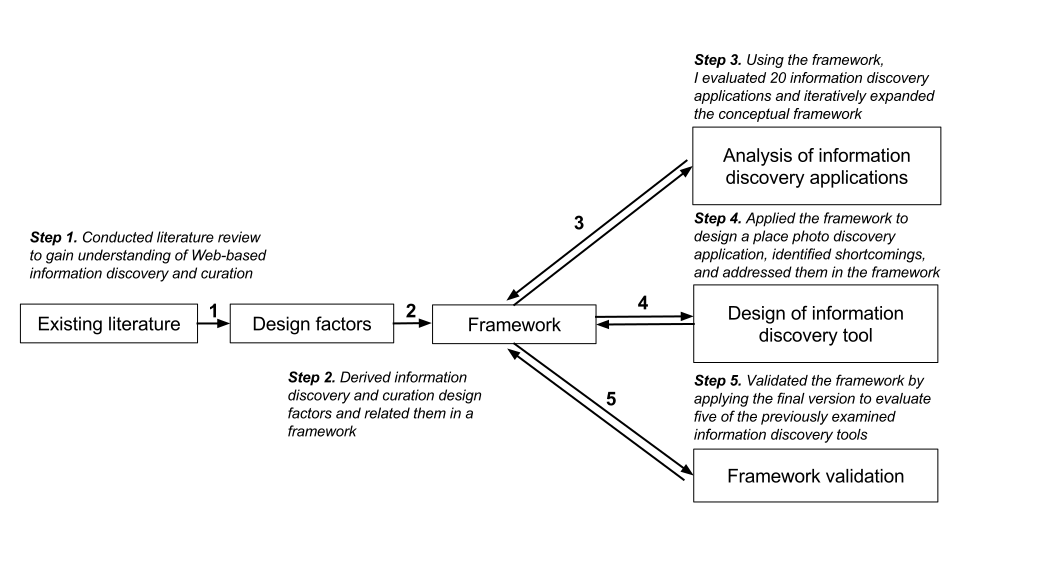
\includegraphics[width=\linewidth]{Methodology.png}
	\caption{Methodology Overview}
	\label{fig:methodology} 
\end{figure}

{\section{Research Questions}
This study is designed to address the problem of designing for information discovery, and it is motivated by the following research questions:

\emph{RQ1: How do existing Web applications support information discovery?}

\emph{RQ2: How do existing information discovery applications support information curation?}
}% end section

{\section{Literature Review}
Development of the framework began with an extensive literature review. A diversity of topics contributed to forming an understanding of information discovery and curation, including information behaviour and information seeking models, high-level Web tasks and modes of Web use, exploration-based models of discovery, and methods of personal and social curation. From this review, the preliminary design factors for the framework were derived. Key findings in current literature are presented in Chapter~\ref{chapter:chapter_related_work}.
}% end section

{\section{Building and Refining \\the Conceptual Framework}
Through a careful analysis of 20 information discovery applications (see Table~\ref{table:tools}), the framework was iteratevely expanded by adding new concepts and establishing relations between those concepts.  The framework was refined as I explored the literature and available tools, and for presentation purposes int his thesis, I present only two versions of the framework. The first preliminary framework was a result of this tool analysis, and it is depicted in Chapter~\ref{chapter:old_framework}. The final version of the framework (see Chapter~\ref{chapter:framework}) was a result of developing an information discovery application based on the preliminary work.    

For the case study, I selected the most popular information discovery applications in use today and considered the full range of features in those tools (both by referring to the literature and documentation on those tools, as well as exploring the features). The popularity of information discovery applications was determined using Website popularity ranks provided by Alexa\footnote[1]{Alexa is available at www.alexa.com}, a commercial Web traffic data provider. The focus was on applications that had strong information discovery components and lesser priority was given to applications whose purpose revolved only around curation.

I used Yin’s strategies for designing a case study~\cite{yin2014case} for guidance. The motivation behind choosing a case study over other methods of qualitative research was based on my choice of research questions (which have an explanatory nature), the lack of control over existing applications and their development, and having to focus on contemporary use of real-life Web applications. According to Yin~\cite{yin2014case}, a case study would be an optimal research strategy given the above characteristics.

For each case of my study, I chose a Web application whose primary purpose is to support information discovery. I examined the overall purpose of each application, its description as defined within the application, and literature and documentation related to the application (if they were available) against the features that the application provided. For example, if an application provided bookmarking features, I checked if it was indeed intended to be used for information preservation. 

Consequently, the methodology was an iterative process of selecting cases, analyzing them, and determining whether they could be described and evaluated using the framework. If I found a key feature that could not be described, I adapted the framework according to the findings. I repeated the process of case selection and evaluation until the framework was usable for all cases. I then grouped the elements of the framework into categories, recording corresponding questions to ask in order to evaluate applications. 

A list of the tools that were used as cases as well as identifying descriptions for each tool are presented in Table~\ref{table:tools}. Other tools were considered throughout the study, however, only the 20 applications presented underwent systematic examination. 

\begin{table*}[htbp]
\small
\label{table:tools}
\caption{Web-based Information Discovery and Curation Tools}

\begin{tabular}{|p{0.20\linewidth}| p{0.30\linewidth}| p{0.45\linewidth}|}

\hline
Application     & Address 	& Description                                                                                                                                                                                                                                                                                            
\\
\hline
Pinterest       & www.pinterest.com 	& Visual discovery tool \\
\hline
Delicious       & delicious.com 		& Social bookmarking service \\
\hline
Tumblr          & www.tumblr.com 		& Microblogging platform \\
\hline
StumbleUpon     & www.stumbleupon.com  	& Web page discovery tool \\
\hline
Wikipedia       & en.wikipedia.org   	& Free content Internet encyclopedia\\
\hline
Google Maps     & www.google.ca/maps  	& Web mapping service\\
\hline
Rotten Tomatoes & www.rottentomatoes.com & Movie and TV database\\
\hline
500px           & 500px.com            	& Photography site\\
\hline
BucketList      & bucketlist.org  		& Goal tracking and discovery service\\
\hline
We Heart It     & weheartit.com 		& Visual discovery tool \\
\hline
Scoop.it!       & www.scoop.it 			& Online publishing platform \\
\hline
Google Images   & images.google.com  	& Image discovery service \\
\hline
Vimeo           & vimeo.com  			& Video sharing Website\\
\hline
LifeHacker      & lifehacker.com        & Daily blog \\
\hline
YouTube         & www.youtube.com 		& Video hosting platform \\
\hline
Yelp            & www.yelp.ca  			& Business review site\\
\hline
IMDb            & www.imdb.com  		& Movie database \\
\hline
Trip Adviser    & www.tripadvisor.ca 	& Travel site \\
\hline
Urban Spoon     & www.urbanspoon.com    & Online bar and restaurant guide\\
\hline
Thesaurus       & thesaurus.com         & Online thesaurus \\
\hline
\end{tabular}
\end{table*}

} % end section

{\section{Applying the Framework to Design\\ an Information Discovery Application}
In order to analyze the framework's capabilities in design for information discovery and curation, I used the framework as a guide for developing a place photo discovery application. Applying the framework to design an application has triggered more changes within the framework, its further extension and refinement. The resulting application is discussed in Chapter~\ref{chapter:application}.
}% end section

{\section{Framework Validation}
In order to finalize the framework, it was applied to reevaluate five of the previously examined tools (see Chapter~\ref{chapter:application}). For each tool, I identifies gaps and proposed directions for future development. 
}% end section

{\section{Limitations}
The case study I conducted has a number of limitations: a lack of documentation, literature, and formal descriptions of available features for some applications introduces a threat to the construct validity of the study. In addition, information discovery tools and features can be used in manners unintended or unforeseen by designers and developers. Therefore, the use of some features within information discovery applications was recorded based on my interpretations. To compensate for such limitations, I employed the tools for personal use over an extended period of time to gain a deeper understanding of their use. In addition, I considered some cases with repeating functionality and design to be able to validate or clarify prior findings. 

Many Web applications rapidly evolve. Therefore, my tool analysis only applies to tools at the moment of the study.

Only Web applications running in browsers on a desktop computer were considered in this study. The study can be extended with use of various devices, such as smartphones and tablets, as information discovery patterns and mechanisms may very for different platforms. 

Another limitation was the lack of prior research studies on the subject matter. Some researchers have studied information seeking models and high-level Web tasks, but there is a lack of literature on how to enable and support different Web tasks. This opens up opportunities for future research to analyze methods of developing and building frameworks for facilitating and evaluating tools that support other Web tasks, such as communication, transactions, and goal realization.


} % end section


\chapter{Web-based Information \\Discovery and Curation}
\label{chapter:chapter_related_work}

Given the complexity of Web-based information discovery and curation tasks, a variety of topics was examined to gain an understanding of how current Web tools support these tasks, including known characteristics of information-related Web usage, currently existing information behavior models, and other aspects of information discovery and curation.  This chapter outlines the key background literature that contributed to the development of the conceptual framework and helped answer the research questions. 

{\section{Information Behavior}
As defined previously, information behavior refers to the totality of ways in which humans behave in relation to information~\cite{wilson2000human}.  A number of models and frameworks were proposed to represent human information behaviour in its entirety or to represent some of the components, such as information seeking, information discovery, and information curation. 


{\subsection{Information Behavior Models}
One of the early information behavior models was proposed by Wilson~\cite{wilson1981user} in 1981. According to the original model, information seeking behavior results form the user trying to satisfy their perceived information need. Consequently, the user makes demands on information systems. Success or failure of such demands dictates whether the process is repeated or, if the information need is satisfied, used or communicated with other people. 

In addition, Wilson defined possible barriers that can impede information seeking behaviors, as well as context that influences formation of the information need. These underlying ideas remained in the revision of Wilson's model ~\cite{wilson1997}.

Finally, Wilson proposed a "problem solving model" of information seeking behavior. The model reflects on the idea that people engage in information seeking and searching in order to resolve some uncertainty that stands in the way of solving, defining, or identifying a problem.    

} % end subsection

Ellis et al. ~\cite{ellis1989, ellis1997, ellis1993} proposed a model of information seeking characterized by six different patterns: starting, chaining, browsing, extracting, monitoring, and differentiating. Subsequently, Choo et al. ~\cite{choo} derived anticipated Web tasks that correspond to these patterns. According to the authors, when users identify sources of interest, they usually identify which Websites can point to that information of interest.  Chaining occurs when users navigate through links on those initial pages. When people browse, they scan top-level pages, headings, lists, and site maps. Differentiating takes place when people bookmark, print, copy and paste information, or choose an earlier selected site. Monitoring occurs when users revisit Web pages or receive updates from previously visited sites. Finally, extraction can occur when the user systematically searches sites to extract information of interest. Ellis' model also complemented Kuhlthau's ~\cite{kuhlthau} work which corresponded stages of information seeking with feelings, thoughts, actions, as well as anticipated information tasks.

Information retrieval behaviors are further studied by Saracevic ~\cite{saracevic} and Ingwersen ~\cite{ingwersen} who derived models concentrating on cognitive processes of information seeking. 
 
Bates ~\cite{bates1986} proposed a model of four information seeking modes: being aware, monitoring, browsing, and searching. Bates differentiated the modes based on the user's level of attention being active or passive, and information needs being directed or undirected. Thus, browsing can be characterized as undirected active information seeking because users do not know directly what information they are looking for, but they are actively looking. Searching falls under active directed information seeking because the information need is clearly defined and the search is directed. Finally, monitoring and being aware are passive modes of information seeking although monitoring is directed and being aware is undirected.

} % end subsection
   
{\subsection{Digital Curation}

In 2002, Bates ~\cite{bates2002} extended her research with the notion of information farming, which involves people collecting and organizing information for future use and revisitation. More commonly, information farming is referred to as digital curation, which is the notion of collecting and managing digital information for the purpose of adding value to the collection and revisitation ~\cite{beagrie}. Wittaker ~\cite{wittaker} believes that in terms of Web use, a significant shift is happening from information consumption to information curation, which means that people no longer just use the Web to find and consume the information that they are interested in, but they also try to save and manage that information so that it can be reaccessed and exploited later. 




{\subsection{Information Exploration Frameworks}



}

{\subsection{Information Discovery Frameworks}



}


{\section{Web Tasks and Modes of Web Use}
The other body of work besides cognitive models and frameworks for information behavior looks at information discovery and curation in term of web use tasks or methods that people employ.

Kellar et al.~\cite{kellar2006goal} separated Web tasks into five categories: transactions, browsing, fact finding, information gathering, and other uncategorized tasks, with information seeking being composed of browsing, fact finding, and information gathering. Although the authors categorized information gathering as part of information seeking, it is in fact more closely related to digital curation ~\cite{beagrie, wittaker}. In their later work, Kellar et al.~\cite{kellar2007field} added communication and maintenance as additional Web tasks. 

Similarly to Kellar et al., Sellen et al. ~\cite{sellen} identified six tasks that are commonly performed by Web users: browsing, finding, housekeeping, information gathering, communicating, and transacting. Therefore, Kellar et al. and Sellen et al. both identified browsing, fact finding, and information gathering as information-related tasks that users perform online.   

People often engage in information seeking activities to close some knowledge gap that occurred as a result of not having enough information to perform a task ~\cite{proper}. Therefore, when providing tool support for various information discovery tasks, it is useful to consider the motivation behind these tasks as it can be different for each task. Morrison et al. ~\cite{morrison} make a distinction between methods of Web use and purposes. The authors derived a purpose-based taxonomy of Web use, including three purposes or motivations: finding information, comparing pieces of information or choosing products to make a decision, and using the Web to find relevant information to gain an understanding of some subject. Consequently, methods of finding information identified by Morrison et al. are collecting, finding, exploring, and monitoring. The differences between the two taxonomies suggest that different information seeking tasks may be performed to satisfy more than one information seeking purpose. Therefore, each purpose may require more than one task-supporting mechanism. 

Morrison et al. also draws distinction between finding or looking up information and exploratory search. Whereas information lookup involves tasks such as fact retrieval, navigation, and verification, exploration is more cognitively demanding and involves learning and investigation ~\cite{marchionini}. Learning and investigation can be performed over multiple iterations, and can involve learning though various media, "social searching", and serendipitous browsing performed with the goals of knowledge acquisition, socialization, forecasting, and planning.  

Categorizing Web usage into information seeking, digital curation, and other Web tasks does not necessarily give full insight about how information-related tasks are performed. Lindley et al. ~\cite{lindley} conducted a qualitative study involving 24 participants, tracking their daily Web usage in the form of a diary. As a result of this study, the researchers identified five distinct modes of Web use: respite, orienting, opportunistic, purposeful, and lean-back. According to the authors, people browse the Web \textit{opportunistically} when they look for information related to some personal interest, long-term goal, or future ambition. \textit{Purposeful use} occurs when the users know what information they need to acquire or what online action they need to perform in order to continue or finish some other activity. \textit{Respite} mode usually occurs when users are in the process of waiting for something or taking a break, and it serves as a means for people to temporarily occupy themselves when high engagement with the content is not a requirement. \textit{Orienting} mode usually occurs when people want to be updated on what has been happening in their environment. Examples of this mode are checking email at work or looking at the news and updates on a social networking site. Finally, \textit{lean-back} mode of Web use can be thought of as listening to the radio or watching television, and usually involves watching videos online or browsing through other types of entertainment content. 

Lindley et al.'s primary motivations behind looking at use modes that occur when people browse the Internet was that traditional Web use studies and Web tasks discovered by other researchers cannot reflect the depth of user's intentions online. Understanding the characteristics of different modes guides the design of Web interaction. For example, opportunistic use can have blurry and continuously changing information needs. People often cannot indicate the completion of Web tasks, and they finish whenever they have been browsing the Internet for too long, or whenever they need to complete some other task of higher priority. Then, they will often resume their opportunistic information seeking. Finally, opportunistic use is 'grasshopper-like', which means that users jump from one resource to another ~\cite{lindley}. From these factors, we can assume that to support such Web usage, we would need to consider mechanisms for supporting users' information needs and support revisitation and arbitrary navigation.

} % end subsection

{\section{Collaborative Information \\Discovery and Curation}
By surveying 204 Web users, Morris found that people often desire to or do collaborate on information seeking tasks ~\cite{morris}. To collaborate on information seeking, people often use instant messaging, email, and create documents and Webpages to share information. Occasionally, collaborative information seeking occurs when collaborators work side by side and share search results in person.

Collaborative information-related activities on the Web are not limited to information seeking. Collaborative information tagging is a way of organizing content for future search and navigation. Although it is usually performed for personal reasons, tagging greatly enhances information retrieval ~\cite{golder}.

} % end subsection

Today, there are a multitude of tools that support different aspects of information exploration and curation, but understanding how these tools are similar (or differ) is difficult. Moreover, the existing research is not useful at helping identify gaps in current tools or ways that current tools may be improved to support information
exploration and curation. Thus, we present a framework of Web application design factors and questions that facilitate information discovery and curation (see Sec. 4).
       
\chapter{Preliminary Framework}
\label{chapter:old_framework}
The preliminary framework was designed with the goal to support information discovery and curation~\cite{voyloshnikova2014}. The framework is presented in Tables~\ref{}, with the goal to illustrate how the framework evolved.

{\section{Framework Composition}
The framework was built by combining the mechanisms based on the literature.

\textit{Serendipitous discovery} refers to information discovery resulting from serendipitous browsing. Such discovery is characterized by under-defined, absent, or hidden information needs, and it usually involves browsing through diverse resources with varying content types ~\cite{kellar2006, kellar2007}. Here, resource is defined as a collection of information about a single unit of inquiry, usually bundled together for presentation purposes. Some examples of resources are places, images, blog posts, and Web pages.

\textit{Fact discovery} refers to information discovery resulting from the search for a specific piece of information. It is characterized by a well-defined information need and is easier to perform within systems that provide access to homogeneous types of information ~\cite{kellar2006, lindley}.

\textit{Rediscovery} refers to information discovery resulting from revisiting previously discovered resources ~\cite{tauscher}. The following is a list of factors that enable rediscovery.

\textit{Channel-based discovery} can incorporate two different information seeking tasks, monitoring and awareness. It occurs when information is suggested to users based on the content that they are subscribed to. If users can actively look for updates, then an application affords monitoring ~\cite{morrison}. If users can receive notifications about updates, then an application facilitates awareness ~\cite{bates2002, bates1986}. Channel-based information discovery is usually enabled at sites that have regularly updated content, such as Pinterest and YouTube.                            

} % end section
{\section{Discussion}
Although the preliminary framework was good at breaking down the tasks that people perform when discovering information, some of the aspects require clarification. 
} % end section


\begin{table*}[htbp]
\caption{Preliminary Framework - Discovery}
\centering

\footnotesize
\begin{tabular}{|p{0.31\linewidth}|p{0.64\linewidth}|}
\hline
\textbf{\small{Design factors}}   & \textbf{\small{Questions to be posed during the design or evaluation of Web-based information discovery tools 
}}  \\
\hline
\emph{\textbf{Serendipitous discovery}}     &                                                                                                           \\

Arbitrary navigation         & Does the application provide a means for arbitrary navigation among resources?                              \\
Search-based navigation      & Does the search engine help retrieve diverse resources related to the topic of interest?               \\
Category-guided navigation & Do categories suggest and help with navigating to resources related to the topic of interest?           \\
Integration                  & If resources originate from a different site, do they link to their original sources?                   \\
Visual link preview               & If resources are delivered as links, do they have visual previews?                                                                        \\
Spatial arrangement          & Is there a semantic to the spatial arrangement of resources?                                                    \\

\emph{\textbf{Fact discovery}}                &                                                                                                           \\
Search-based navigation      & Does the search feature help discover the specific resource of interest?                                  \\
Category-guided navigation & Do categories help narrow results to specific types of resources?                                   \\
Integration                  & If resources originate from a different site, do they link to their original sources?                   \\
Uniform representation       & If resources are uniform, are they presented in a uniform way? \\
Visual link preview               & If resources are delivered as links, do they have visual previews?                                                                        \\
Spatial arrangement          & Is there a semantic to the spatial arrangement of resources?                                                    \\

\emph{\textbf{Rediscovery}}                     &                                                                                                           \\
History-based rediscovery    & Does the application save and provide access to browsing history?                                        \\
Bookmark-based rediscovery   & Does the application support bookmark-based resource revisitation?                                        \\
Search-based rediscovery     & Is the search a reliable method for resource revisitation?                             \\

\emph{\textbf{Channel-based discovery}}          &                                                                                                           \\
Site subscription            & Does the application allow subscriptions to news and updates?                                             \\
User subscription             & Does the application allow subscriptions to other users' activities?                                      \\
Notifications                & Does the application have one or more notification mechanisms?                                                      \\
Subscription to news feed                  & Can subscription updates be visible within the application?  \\
Content news feed                  & Can content updates be visible within the application? \\

\hline     

         
\end{tabular}
\end{table*}


\begin{table*}[htbp]
\caption{Preliminary Framework - Curation}
\centering
\footnotesize
\begin{tabular}{|p{0.25\linewidth}|p{0.65\linewidth}|}
\hline
\textbf{\small{Design factors}}   & \textbf{\small{Questions to be posed during the design or evaluation of Web-based information discovery tools 
}}  \\

\hline          
\emph{\textbf{Management}}                    &                                                                                                           \\
List-based categorization               & Does the application support sorting information into list-like structures, either privately or publicly?                                                  \\
Tag-based categorization               & Does the application support tagging, either privately or publicly?                                                  \\

\emph{\textbf{Preservation}}                   &                                                                                                           \\
Internal preservation of internal resources       & Does the application support bookmarking mechanism(s) for preserving internal information within the application?        \\
Internal preservation of external resources       & Does the application support bookmarking mechanism(s) for preserving external information within the application?        \\
External preservation of internal resources      & Does the application support bookmarking mechanism(s) for preserving internal information outside of the application? \\ 

\emph{\textbf{Augmentation}}            &                                                                                                           \\
Evaluation                   & Can the resource evaluations be recorded privately or publicly? \\
Annotation                   & Can resources be annotated privately or publicly?                                                                               \\    
       
\emph{\textbf{Sharing}}            &                                                                                                           \\
Adding resources             & Can resources be publicly added to the collection of information within the application from other Web pages?     \\
Internal sharing         & Can internal resources be publicly reshared within the application?         \\ 
External sharing          & Can internal resources be publicly reshared outside of the application?         \\ 
         
\hline
\end{tabular}
\end{table*}






\chapter{A Conceptual Framework for Information Discovery and Curation on the Web}
\label{chapter:framework}

Although Web-based information discovery and curation tasks are commonly performed today, as we mentioned above, there is a lack of literature on how to enable and support them when building Web applications. I reduce this gap by presenting a framework of design factors facilitating digital information discovery and curation. 

In my framework, I built on existing models and frameworks of information discovery and curation and analysis of existing Web tools to derive corresponding design factors for Web design. I borrow terminology from Activity Theory~\cite{kuutti1996activity} to describe how different components of the framework are connected. 

The framework is divided into two parts. This chapter outlines the first part of the framework titled \textit{``Enabling Information Discovery and Curation''}. The first part of the framework consists of motives behind information discovery and curation, actions that discovery and curation consist of, and design factors that enable those actions (see Figure~\ref{fig:framework_part1}). Second part of the framework deals with improving operations that are involved in information discovery and curation (see Chapter~\ref{chapter:improving}).

\begin{figure}[ht!]
	\noindent
	\centering
	\includegraphics[width=\linewidth]{framework_part1.png}
	\caption{Framework Overview (Part I): Enabling Information Discovery and Curation}
	\label{fig:framework_part1} 
\end{figure}

{\section{Motives Behind Information Discovery and \\ Curation}
Understanding the motives behind user activities can help form a conceptual model of a needed Web application and its features. There exists a wide variety of user motives behind information discovery and curation, and certain aspects of these motives can significantly impact the design of an application. The following generalizations of motives and their properties can help define conceptual models and identify primary use cases of Web tools for information discovery and curation.  

{\subsection{Closing Knowledge Gap}
The primary motive for information discovery is usually to close a knowledge gap that occurs when the user tries to accomplish a task and lacks information to do so. This motive can take up various forms. Its form commonly depends on the nature of an information need and other conditions surrounding the given motive.        

Depending on the context in which it arose, an information need can have various degrees of specificity. For example, if the motive is to find inspiration for a project, an information need is only vaguely defined. However, if the motive is to find a phone number of a specific business, an information need is well-defined. In some cases, the information need may be hidden, and the user might not be aware of the existing knowledge gap. The specificity of an information need determines important properties of information discovery mechanisms, such as whether users can benefit more from mechanisms that allow to specify an information need, help form an information need, or allow to randomly retrieve information. This property has to be taken into consideration when evaluating or designing a Web application. 

The nature of an information need predetermines whether discovery is respectively serendipitous or oriented towards fact finding. Therefore, depending on user needs, an application can be designed to increase serendipity and opportunistic discovery or to improve purposeful fact finding. For instance, displaying featured content can improve serendipitous discovery because of its inconsistent nature and novelty. Using context, such as location and date, to tailor search results to the user can improve fact finding. 

The motive behind information rediscovery involves finding previously discovered information and closing previously closed knowledge gap in case if information was forgotten. It usually results in the user looking for previously found resources and Web pages. In fact, Web-page revisitation is one of the most commonly performed web-browsing activities~\cite{adar2008large,cockburn2003improving}. The percentage of revisited web pages involved in web browsing can range from 58\%~\cite{tauscher1997people} to 81\%~\cite{cockburn2001web}. Some of the reasons for revisiting pages include shopping, communication, entertainment, education, activity planning, and hobby-related information retrieval~\cite{adar2008large}. Some Web pages and resources can be rediscovered using navigation while others need to be previously preserved (bookmarked) in order to allow rediscovery. Rediscovery is one of the many ways in which information discovery and curation interweave. 

Another type of motive for information discovery relates to the two qualities of the Web defined by Lindley et al. - temporality and persistence~\citep{lindley2012s}. \textit{Persistence} refers to the quality of the Web that allows people to habitually revisit Web pages and continue on-going Web projects. \textit{Temporality} refers to the quality of the Web that allows the content of websites to be continuously updated to provide users with new information. Persistence alone usually facilitates information rediscovery. However, if persisitence is combined with temporality, they can facilitate discovery of new information within the same application or channel. I refer to this type of discovery as \textit{channel-based discovery}. Some of the common motives for channel-based discovery include orienting (or monitoring for updates) and opportunistic information discovery~\citep{lindley2012s}.          
}

{\subsection{Future Use and Reaccess}
The main motive behind information curation is to make it possible to retrieve information and to consequently use it. In order to facilitate easy information retrieval, many Web applications employ various forms of bookmarking systems. Traditionally, bookmarks are manually organized by users into folders. However, this method of organization has been found inefficient because folders with bookmarks become easily cluttered~\cite{abrams1998information}. Therefore, in order to efficiently support information rediscovery, Web tools need to provide mechanisms for information preservation along with information management.
}

{\subsection{Improving Collection}
Reportedly, people gather information to improve existing collections~\cite{lindley2012s}. Although some deeper motives may include self reflection or the possibility of future use, collecting information is a motive in itself. In general, information gathering may be stretched over a period of time~\cite{kellar2006goal}, resulting in repeating page visitation. Although information gathering composes only 13.4\% of Web usage, it highly contributes to various goal-supporting activities, such as decision making and planning~\cite{kellar2006goal}.

}

{\subsection{Communication}
As part of his information behavior model, Wilson identified communication of information as an outcome of information seeking. Communication can also be thought of as a motive for information discovery and curation. To support communication of information, Web tools have to provide mechanism that allow various users to share information among themselves. 

In recent years, social bookmarking, a way to preserve and share information within various communities, has gained popularity as an effective way of communicating with other users~\cite{estelles2010social}. One of the first visions of social bookmarking was associated with Web blogging. Oravec~\cite{oravec2002bookmarking} believes that web blogs help annotate or bookmark important information and build a ``map'' of the Internet. Evolution of social bookmarking has advanced bookmarking technologies and provided a means for collaborative information discovery and curation. 
}

Even though it is not entirely feasible to list all of the possible motives for information discovery and curation, in this section I outline some of the important motives and their aspects that can aid in developing use cases and formalizing conceptual models for Web applications. These motives also make it easier to showcase how mechanisms for discovery and curation complement each other. 
}

{\section{Discovery and Curation Activities, Actions, and Their Enablers}
The next portion of the framework consists of two main categories (discovery and curation) that are consequently decomposed into different actions (see Figure~\ref{fig:enablers}). Each of the actions is supported by a group of features or mechanisms that enable given aspect of discovery or curation in a Web application.  The following subsections describe each of the groups and outline corresponding questions that can help application design and evaluation.  

\begin{figure}[ht!]
	\noindent
	\centering
	\includegraphics[width=\linewidth]{framework_enablers.png}
	\caption{Enabling Information Discovery and Curation: Activities, Actions, and Corresponding Enablers}
	\label{fig:enablers} 
\end{figure}

{\subsection{Navigation in Discovery: Following Information Scent}
In order to discover information, a user needs to have a way of navigating to it. Navigation in information discovery can be thought of as following an information scent. In general, information scent models deal with how the users identify value, cost, or access path of information sources based on proximal cues, such as links, icons, categories, etc.~\cite{pirolli1999information}. Common methods of navigation that facilitate information discovery include descriptional, referential, opportunistic, and system-regulated (see Table~\ref{table:navigation}). 


\begin{table}[ht!]
\caption{Navigation Mechanisms}
\label{table:navigation} 
\begin{tabular}{{|p{0.33\linewidth}|p{0.67\linewidth}|}}
\hline
Navigation mechanisms     	& Questions to be posed during the design or evaluation of  discovery and curation tools \\
\hline
\textbf{Descriptional} 			& \\
Search-based navigation							& Is it possible to navigate within the application using a search mechanism? \\
Integrated search				& Is it possible to retrieve information from  other applications using a search mechanism? \\
\textbf{Referential}       		& \\
Categories				 		& Is it possible to navigate using categories? \\
Facets				    		& Is it possible to navigate using facets? \\
Filters					  		& Is it possible to navigate using filters? \\
Tags				      		& Is it possible to navigate using filters? \\
Search by item or resource		& Is it possible to search by item or resource? \\
Integrated reference			& Is it possible to retrieve information from other applications using any of the referential mechanisms?\\
\textbf{Opportunistic}          & \\
Opportunistic navigation        & Is it possible to opportunistically navigate through information within the application? \\
Integrated opportunistic navigation        & Is it possible to opportunistically retrieve information from other application? \\
\textbf{System-regulated}            		& \\
Static direct display           & Is it possible to view static information directly without active search? \\
Integrated static display   	& Is it possible to view static information from other applications without active search? \\
Featured content             	& Is it possible to view featured content? \\
Integrated featured content     & Is it possible to view featured content from other applications? \\
News feed             			& Is it possible to view news feed? \\
Integrated news feed            & Is it possible to view news feed from other applications? \\
\hline
\end{tabular}
\end{table}

{\subsubsection{Descriptional Navigation}
A navigation is descriptional when the user has a means of describing their information need. Most commonly it is implemented as search-based navigation since it allows users to enter the search query and describe what they want to find. Some of the modern descriptional navigation systems can be activated using voice. 

Almost every present-day Web application has the search feature implemented, with rare exceptions of applications that utilize other methods of navigation, such as StumbleUpon and certain shopping websites. Some Web applications are integrated with others enabling users to search multiple websites at once.    

There exist numerous ways in which descriptional navigation supports information discovery. Search-based navigation often serves as an entry point for information seeking~\cite{levene2011introduction}. When the motive behind information discovery has a well-articulated information need, then the user can express their information need by entering a search query. 

Descriptional navigation can also help to rediscover information. However, it is not always a reliable way of refinding information ~\cite{cockburn2003improving}. In information portals that provide access to fairly ambiguous information and that have regularly updated information flow, the search feature is usually designed around retrieving information related to some general topic. In order to make search-based navigation a reliable way to rediscover information, it must return consistent results. 
} % end subsection

{\subsubsection{Referential Navigation}
A navigation is referential when the user finds a reference, such as link or icon, to the term that they are looking for. This reference represents an information scent. The underlying assumption of this method of navigation is that the user can recognize needed information or a reference to it as they see it~\cite{waterworth1991model}. 

Referential navigation mechanisms can take many different forms. Some common types are categories, facets, filters, and tags. In some applications, users can search by a given resource. For example, YouTube provides a playlist with music related to the currently playing song. Information scent representatives may also reference sources outside of the given system. This enables another type of integration of Web applications. 

Referential navigation can help the user identify their information need by suggesting terms, topics, or categories to use, and therefore, directing the user to relevant resources~\cite{levene2011introduction}. It can also help narrow the results to a specific type of resource so that further discovery is bounded by that type. For example, TripAdvisor allows the user to choose among hotels, flights, vacation rentals, restaurants, and destinations, so the application helps to narrow search results.

} % end subsection

{\subsubsection{Opportunistic Navigation}
Opportunistic navigation is method of navigating ``randomly" though resources and Web pages.  As expected, this type of navigation is not authentically random; therefore, I apply the term ``opportunistic" to describe this type. However to the user, this navigation type appears to be randomized, and it promotes serendipitous discovery. This method is especially useful when the information need is fully undefined.

Many applications, such as StumbleUpon and Wikipedia, support opportunistic navigation to allow for opportunistic jumping from one resource to another. StumbleUpon makes it possible to explore the Web in general - other websites and Web applications, allowing for integrated navigation, whereas Wikipedia provides opportunistic access to its own articles. 
} % end subsection

{\subsubsection{System-regulated Navigation}
Often, Web applications display or update information without the user's active participation. This information can be news feed, featured deals or articles, static information, or other types of content. In my thesis, I refer to this type of navigation as system-regulated because it occurs when the application brings the content to the user instead of the user applying any effort to find it. It differs from opportunistic navigation because the the user cannot choose when to observe new information; instead, all updates are regulated by the application. 

One example of an application that utilizes system-regulated navigation is Yelp. This tool displays featured restaurants as well as its user's recent activities as soon as the user enters the site. As any other navigation method, this method can ensure cross-application integration by displaying content from other Web applications. 
} % end subsection
} % end section

{\subsection{Exploration and Discovery}
Exploration of resources is another factor that enables information discovery. In particular, visual and spatial explorations of single or multiple resources allow for rapid information searching (see Table ~\ref{table:exploration}). 

Abrams et al.~\cite{abrams} identified link representation as one of the problems with traditional bookmarking. Analogous with browsing through a bookmark manager, identifying relevant information when browsing through links to diverse resources can be a challenging task. A visual preview should make it easier to evaluate the relevance of resources. Applications that facilitate serendipitous information discovery often employ elaborate resource representation techniques. Many social bookmarking systems, such as Scoop.it! and StumbleUpon, support visual previews of bookmarked pages. Delicious is a social bookmarking application that lacks this type of link representation support, which makes it harder to determine if the link will lead to a relevant resource.

Similar to link representation, spatial visualization of numerous links is another problem that occurs when browsing through diverse content ~\cite{abrams}. Therefore, a semantic to the spatial arrangement of resources is of major importance. Information discovery applications that support serendipitous discovery often have a special way of spatially arranging resources to make it easier to browse through large amounts of information. For example, many tools use a 'pinboard' layout of resources similar to Pinterest.

\textbf{Uniform representation.} Uniform representation is a method of displaying diverse resources in a common way, with each resource having the same set of components ~\cite{herrera}. Such a representation assures that each resource has the same set of facts associated with it, and therefore, the user can afford to have expectations about information that can be found when looking for a specific fact. For example, Yelp displays rating, price range, and address for all restaurants, so not only is it easy to find specific information, but the user can have expectations about the content of resources within the application. On the contrary, searching Tumblr for a restaurant will return a chaotic collection of information about the place. 



\textbf{Visual link preview.} If an application provides links to resources, a visual preview makes it easier to recognize the relevance of the resource ~\cite{abrams}. Applications that support fact discovery often use visual link preview, similar to applications that support serendipitous browsing. However, the motivation behind having a link preview for fact finding is to make it possible to identify if the resource is indeed what the user is looking for. For example, searching for an actor in IMDb will return a list of actors and their photographs, so that the user can pick the one they are interested in.

\textbf{Spatial arrangement.} Similar to serendipitous information discovery, spatial arrangement of resources is important ~\cite{abrams} as a poor semantic to the arrangement can make it difficult to visually navigate to the facts of interest.

\begin{table}[ht!]
\caption{Visual and Spatial Exploration Mechanisms}
\begin{tabular}{{|p{0.33\linewidth}|p{0.62\linewidth}|}}
\hline
Exploration mechanisms & Questions to be posed during the design or evaluation of discovery and curation tools  \\
\hline
\textbf{Visual and textual cues of multiple resources} & \\
Visual preview  & Are there visual previews of resources to help identify resources of value? \\
Textual preview & Are there textual previews of resources to help identify resources of value? \\
\textbf{Visual and textual cues of a single resource} & \\
Visual cues                 & Are there visual cues to help identify the value of information within a resource? \\
Textual cues                & Are there textual cues to help identify the value of information within a resource? \\
\textbf{Spatial proximal cues of multiple resources} & \\
List  						& Are resources presented in a list? \\
Grid   						& Are resources presented in a grid? \\
Gallery  					& Are resources presented in a gallery layout? \\
Spatial semantic            & Is there a semantic to the spatial arrangement of multiple resources? \\ 
Consistency				 	& Are resources presented in a consistent way? \\                                                    
\textbf{Spatial proximal cues of a single resource} & \\
Spatial semantic            & Is there a semantic to the spatial arrangement of information within a resource? \\
Consistency   				& Are same types of resources presented in a consistent way?\\                                                       
\hline
\end{tabular}
\end{table}


} % end section
{\subsection{Integration}

Similar to serendipitous discovery, if an information discovery application provides access to resources from other Websites, the user should be able to navigate to those sites as they may contain the facts of interest. Integration for fact finding is especially important when it gives an opportunity to display specific information about resources that otherwise would not be accessible. For example, Google Maps displays business ratings as a result of its integration with Google+.

To users with ambiguous information needs, one information portal might not provide access to all information of interest. If an information discovery application gives access to resources from various sources, such as other Websites, the user should be able to navigate back to those sources.  
} % end section

{\subsection{Curation}

Information curation is a common activity within many information discovery applications. By asking questions about application design with regards to information curation as in Tables~\ref{table:curation} and~\ref{table:curation_support} of the conceptual framework, designers can find ways to add value to information and enable information exploitation over time.

Information discovery applications vary from being completely socially curated and populated by users, to those that lack any curation mechanisms. 
By definition, digital information curation is the notion of managing, preserving, and adding value to collections of information ~\cite{beagrie, wittaker}. Thus, the curation category consists of information management, preservation, information enhancement, and sharing.


\begin{table}[ht!]
\caption{Curation Mechanisms}
\label{table:curation}
\begin{tabular}{{|p{0.30\linewidth}|p{0.65\linewidth}|}}
\hline
Curation mechanisms  & Questions to be posed during the design or evaluation of  discovery and curation tools  \\
\hline
\textbf{Management} & \\
Collection-based categorization     & Is it possible to sort information into collection-like structures, either privately or publicly? \\
Tag-based categorization          	& Is it possible to tag information, either privately or publicly? \\
\textbf{Preservation} & \\
Internal preservation of internal resources		& Is it possible to preserve internal information within the application? \\
Internal preservation of external resources     & Is it possible to preserve external information within the application? \\
External preservation of internal resources     & Is it possible to preserve internal information outside of the application? \\ 
\textbf{Augmentation} & \\
Annotation & Is it possible to annotate resources, either privately or publicly? \\ 
Evaluation & Is it possible to evaluate resources, either privately or publicly? \\       
\textbf{Sharing} & \\
Adding resources        & Is it possible to add resources to the collection of information within the application from other websites? \\
Internal sharing        & Is it possible to publicly reshare internal resources within the application? \\ 
External sharing        & Is it possible to publicly reshare internal resources outside of the application? \\ 
\textbf{Channel-picking}  	& \\
User subscription       & Is it possible to subscribe to activities of other users? \\
Site subscription       & Is it possible to subscribe to site updates? \\
Artifact subscription  	& Is it possible to subscribe to artifact updates?\\
\hline        
\end{tabular}
\end{table}




{\subsubsection{Management}
Information management is one of the key elements of information curation ~\cite{beagrie, wittaker}. Information categorization mechanisms are prevalent in applications that have a lot of information that is hard to categorize automatically or can mean something different for each user. In the context of Web information management, the following factors play a major role.

Resource categorization helps establish relationships between various resources ~\cite{beagrie, wittaker}. Allowing people to sort information using custom categories can aid rediscovery, discovery in a socially curated space, as well as add more value to resources.

Similar to list-based categorization, tagging aids rediscovery, adds value to resources, and aids discovery, especially in a socially curated space ~\cite{gruber}.  For example, Pinterest supports tag- and list-based categorizations, where lists are represented as 'pinboards'. Tumblr, on the other hand, only supports tag-based categorization. In addition, Pinterest allows for private information categorization.

} % end subsubsection

{\subsubsection{Information Preservation}
Information preservation is a common Web task that is usually performed with the intent of revisiting information ~\cite{abrams, wittaker}. However, in the case of opportunistic Web use, information gathering is sometimes performed with just the goal of collecting information rather than revisiting it in the future ~\cite{lindley}. Bookmarking is a traditional way of preserving information and many Web applications provide diverse bookmarking mechanisms. 

Internal preservation of internal resources means bookmarking resources to be reaccessed within the same application. Such bookmarking facilitates information curation within the system.

Internal preservation of external resources signifies bookmarking other Web pages within an application. 
  
External preservation means bookmarking resources so that they become available through other bookmarking systems. An application must facilitate integration with other applications in order to enable external preservation ~\cite{abrams}.

On We Heart It, users can preserve \textit{internal  information} using \textit{internal collections} and they can add information from \textit{external} Websites. However, there are no integrated means for bookmarking \textit{internal content} using other bookmarking systems.  


Bookmark-based revisitation is one of the most common ways of information rediscovery ~\cite{abrams}. The majority of Web browsers are equipped with bookmarking features. However, some modern Web applications, such as YouTube and Pinterest, provide integrated mechanisms for bookmarking and bookmark-based information rediscovery. 

A Web application needs to automatically record browsing history in order to enable history-based rediscovery ~\cite{tauscher}. History-based rediscovery appears to be the least common rediscovery mechanism, however, it can still be found in some Web applications, such as Google Maps.
} % end subsubsection

{\subsubsection{Augmentation}
One of the most important elements of digital curation is augmentation: adding value to information ~\cite{beagrie, wittaker}. It is often performed within social bookmarking systems. Many Web applications allow users to add value to the resources they curate. 

Evaluation methods can have various forms. They usually take place in socially curated information systems. However, evaluation can also contribute to personal reflection and information preservation. In addition, many applications allow users to evaluate resources by rating them or recording other forms of approval or disapproval. Some sites, such as Wikipedia, do not allow any evaluation. 

Annotations are metadata attached to a resource, such as comments and descriptions. Annotations make it easier to search for and interpret information. 
} % end subsubsection

{\subsubsection{Sharing}
Sharing information is key to empowering social information curation ~\cite{beagrie}. Therefore, the main components that facilitate sharing are adding resources, and external and internal information sharing.

Adding resources not only facilitates global Web information curation, but it also scales the information available through the system, providing more opportunities for information discovery. Resources can be created by users themselves, taken from some other sources online, or both. For example, YouTube allows users to upload their own videos, whereas Pinterest permits adding images from other sites in addition to users' personal images. 

Sharing resources through different media supports channel-based information discovery within the media channels. Information discovery applications commonly allow for sharing information on popular networking sites outside the application.

Resharing resources within the system supports channel-based information discovery. 
} % end subsubsection

{\subsubsection{Channel-picking}

Subscriptions to updates from a site help users follow the news ~\cite{java}. In order to support subscription-based discovery, an application must provide a subscription mechanism. For example, Rotten Tomatoes allows subscriptions to newsletters; however, it does not allow subscriptions to movie critics, as a user-based subscription mechanism would allow. 

In some applications, the content is updated and curated by users, and users can subscribe to other users. Similar to site subscriptions, user subscriptions are subscriptions to activity updates from individual users rather than all content updates, and help with networking and following users' activities ~\cite{millen}. Such subscriptions help to further filter new content delivered to the user. 

Notification mechanisms enable user awareness about new content on the subscribed channel ~\cite{millen}. Different applications provide various notification mechanisms including messages within the application, informative emails, and smartphone notifications.

Displaying a news feed within the application further promotes awareness and can serve as a monitoring mechanism. For such. 

Similar to displaying a subscription news feed, displaying a content news feed promotes awareness and can serve as a monitoring mechanism.

Information discovery and curation tools can have different implementations depending on the motives behind these activities.  

} % end subsubsection
} % end subsection
} % end section











\chapter{Improving Information Discovery and Curation Activities}
\label{chapter:improving}


\begin{figure}[ht!]
	\noindent
	\centering
	\includegraphics[width=\linewidth]{framework_part2.png}
	\caption{Framework Overview (Part II): Improving Information Discovery and Curation}
	\label{fig:framework_part2} 
\end{figure}

{\section{Improving Navigation}
There are two common ways of aiding information discovery when search-based navigation is used. The first method entails returning personalized results when the user enters a search query. There are a number of ways to accomplish personalization, but this chapter only focuses on which features can can support information discovery and curation have rather than their implementations. The second method is to suggest search terms to make it easier for the user to formulate the information need (see Table~\ref{table:navigation_support}).

To further support referential navigation, applications can either personalize search results (similarly to descriptional navigation) or personalize reference suggestions (see Table~\ref{table:navigation_support}). 

To further enhance random navigation, Web tools sometimes allow users to personalize this type of navigation, which makes it less 'random'. However, this way the user can discover new information within a specific category, for example.

Displayed content can also be personalized to improve information discovery with direct navigation.

\begin{table}[ht!]
\caption{Cognitive Support, Automation, and Personalization for Navigation}
\label{table:navigation_support}
\begin{tabular}{{|p{0.35\linewidth}|p{0.60\linewidth}|}}
\hline
Support, automation, and personalization elements & Questions to be posed during the design or evaluation of discovery and curation tools \\
\hline
\textbf{Descriptional}       & \\
Personalized results         & Does the search mechanism return personalized results? \\
Filtered search mechanism    & Is it possible to apply filters to the search criteria? \\
Guided search                & Does the system suggest search terms to the user? \\
\textbf{Referential}         & \\
Suggesting categories & Does the system suggest categories of interest? \\
Suggesting topics of interest & Does the system suggest topics of interest? \\
Suggesting tags              & Does the system suggest similar tags? \\
Suggesting similar resources & Does the system suggest similar resources? \\
\textbf{Opportunistic} & \\
Personalized opportunistic navigation     & Is it possible to personalize opportunistic navigation? \\
\textbf{System-regulated} & \\
Personalized featured content         & Is featured content personalized to the user? \\                                                       
User activity update notification & Is it possible to receive notifications about other users' activities? \\
Application activity update notification & Is it possible to receive notifications about website content updates?\\
Artifact update notification & Is it possible to receive notifications about artifact-related updates? \\                                                       
\hline

\end{tabular}
\end{table}


} % end subsection
{\section{Improving Exploration}

\begin{table}[ht!]
\caption{Visual and Spatial Exploration Cognitive Support and Personalization}
\begin{tabular}{{|p{0.33\linewidth}|p{0.62\linewidth}|}}
\hline
Cognitive support and personalization design elements & Questions to be posed during the design or evaluation of discovery and curation tools  \\
\hline
&\\
\textbf{Visual and textual cues of multiple resources} & \\
Personalized visual preview  & Is it possible to personalize visual previews of resources? \\
Personalized textual preview & Is it possible to personalize textual previews of resources? \\
&\\
\textbf{Visual and textual cues of a single resource} & \\
Personalized visual cues                 & Is it possible to personalize the visual cues within a resource? \\
Personalized textual cues                & Is it possible to personalize the textual cues within a resource? \\
&\\
\textbf{Spatial proximal cues of multiple resources} & \\
Personalized arrangement of multiple resources & Is it possible to personalize the arrangement of resources? \\   
&\\                                                 
\textbf{Spatial proximal cues of a single resource} & \\
Personalized arrangement of information within a resource          & Is it possible to personalize the arrangement of information within a resource? \\                                                       
\hline
\end{tabular}
\end{table}

} % end subsection

{\section{Improving Curation}

\begin{table}[ht!]
\caption{Cognitive Support, Personalization, and Automation for Curation}
\label{table:curation_support}
\begin{tabular}{{|p{0.30\linewidth}|p{0.65\linewidth}|}}
\hline
Cognitive support, personalization, and automation elements & Questions to be posed during the design or evaluation of information discovery and curation tools \\
\hline
\textbf{Management}		& \\
Suggesting collections  & Does the system suggest relevant collections? \\
Suggesting tags         & Does the system suggest relevant tags? \\
Automated classification into collections  	& Does the system automatically sort resources into collections? \\
Automated tagging       & Does the system automatically tag resources? \\
\textbf{Preservation}   & \\
History       			& Does the system automatically preserve information found by the user? \\
Suggested preservation  & Does the system suggest preservation channels to the user? \\
\textbf{Augmentation} 	& \\
Automated augmentation  & Does the system automatically annotate resources? \\
Suggested augmentation  & Does the system suggest annotation options to the user? \\    
\textbf{Sharing}        & \\
Automated sharing		&  Does the system support automatic sharing? \\
\textbf{Subscription}   & \\
Suggesting users for subscription & Does the system suggest which users to subscribe to? \\
Suggesting artifacts for subscription   & Does the system suggest which artifacts to subscribe to? \\
Automatic subscription  & Can the system subscribe the user automatically to the website activity? \\

\hline  
\end{tabular}
\end{table}

Notification mechanisms enable user awareness about new content on the subscribed channel ~\cite{millen}. Different applications provide various notification mechanisms including messages within the application, informative emails, and smartphone notifications.
} % end subsection

{\section{Personalization Strategies}
} % end subsection

Providing cognitive support, personalization, and automation dramatically improves user experience when they interact with information discovery and curation systems. Using the information discovery factors in my framework, I described and evaluated currently existing tools. Similarly, the framework can be used for identifying gaps in information discovery support and developing new technologies (see Chapters~\ref{chapter:application} and~\ref{chapter:evaluation}).  
\chapter{Framework Application}
\label{chapter:application}

To verify that the final version of the framework was effective (see Chapter~\ref{chapter:framework}), I applied it to design a place photo discovery application as well as to reevaluate five of the applications that were used in the construction of the preliminary framework described in Chapter~\ref{chapter:old_framework}. This section outlines application design process, and evaluations of the tools with proposed directions for development of these applications. 

{\section{Design Process}

}%end section

{\section{KeePlaces}
\begin{figure}[ht!]
	\noindent
	\centering
	\includegraphics[width=\linewidth]{keeplaces.png}
	\caption{KeePlaces}
	\label{fig:keeplaces} 
\end{figure}
{\subsection{Navigation}
Descriptional navigation is possible using search. The search feature is not guided, and so far, results are not personalized. 

}
{\subsection{Exploration}
Spatial exploration of multiple resources is enabled through the gallery view. 
Resources are represented as photos, so visual exploration of multiple resources is enabled. However, there is no way of exploring each resource individually, therefore, exploration of a single resource is not supported. 
}
{\subsection{Integration}
KeePlaces is integrated with Google Maps.
}
{\subsection{Curation}
Curation in Keeplaces is supported through management and preservation.

Management is implemented using collection-based classification.
Every photo discovered on the site can be bookmarked, or 'kept', in a collection.
}
{\subsection{Channeling}
Channeling has not yet been enabled within the application, but it is an important aspect behind the conceptual model of the application.
}
{\subsection{Directions for Future Development}
As mentioned above, channeling is the first aspect that needs to be implemented along with enhancing management mechanisms.
}
} % end section





\chapter{Research and Design Implications}
\label{chapter:implications}

The conceptual framework for information discovery and curation is designed to perform formative and summative evaluation of existing Web applications, with a goal to reveal how these tools support information-related activities in question. The framework, as a tool, and its capability to guide the process of analyzing Web applications makes it broadly applicable in research and Web design. 

In Chapter~\ref{chapter:evaluation}, I demonstrate how the framework can be used to reveal missing features in tools. Using similar methods, the framework can also be applied to compare different Web applications. When used for evaluation, the framework helps to identify which areas of a given tool require further attention. Therefore, the framework can be helpful for designers who wish to improve existing tools or get ideas for new information discovery and curation applications. 

Factors and questions of the framework are there to guide the developer, but they do not dictate which features should be in an application. In other words, the framework helps expose gaps, but it is up to designers to decide whether those gaps need to be closed. In fact, some gaps cannot be closed because of certain constraints, such as data type and system design.

User interface designers face certain trade-offs when developing applications. Therefore, it is not always advantageous to implement all of the missing features. For example, providing the support to customize spatial arrangement of multiple resources can undermine the consistency of their representation. 

In the research domain, the framework can serve as a guide for drawing distinctions between different Web-based information discovery and curation applications, finding gaps in tools that can be studied, and selecting cases for studies based of required functionality. Hence, both researchers and developers can benefit from the systematic tool examination guided by the framework.

Even though applying the framework requires initial expertise and critical reasoning, it opens up opportunities for research and practice. Systematic evaluation of Web tools for information discovery and curation helps improve user experience and gain better understanding of information behaviour within a given system. 





\chapter{Future Work and Conclusions }
\label{chapter:future_work}


In our study, we analyzed information curation and seeking tasks and developed a conceptual framework of factors and questions that are important when building and evaluating Web information discovery tools. We then evaluated and iteratively refined the framework by analyzing 20 different information discovery applications and provided concrete examples of tool support addressing various concepts of our framework.

One of the possible future research objectives would be to apply the framework to identify a gap in available information discovery tools, and then further use the framework to design an application that would close that gap. Another potential research question would be to expand our investigation to include the factors that influence the need for one information discovery type over another. 

Our framework opens up opportunities for structured information discovery tool evaluation and design. As more tools are being developed within the social space of information discovery and curation, understanding how these tasks can be supported promises advancements in how Web applications are designed.

Additionally, I would like to investigate how collaboration in information discovery and curation relates to the framework.




\bibliographystyle{apa}
\bibliography{refs}

\appendix              %- maybe some appendices
%\include{app1}
%\include{app2}

%--------------------------------------------------------------
%- Here is a semi-automatic VITA page construction.
%- If you don't like the page layout you have to make your own.
%--------------------------------------------------------------

\vita                  %- This commands starts the vita page(s)

%- Now call \fullinfo with four arguments:
%-    lastname, givenname, birthplace, and birthdate.
%- I think that the birthdate is according to Dec. 1994 rules
%-    is optional.
%- So, I also provide the command:
%-    \halfinfo{lastname}{givenname}{birthplace}


\halfinfo{Voyloshnikova}{Elena}{Nikolaev}

%-
%- Next, the education:
%- \begin{education} ... \end{education}
%- Each entry must be entered as \entry{university}{years}}
%-

\begin{education}
\entry{University of Victoria}{2008 to 2012}
\end{education}

%-
%- Next the degrees:
%- \begin{degrees} ... \end{degrees}
%- Now \entry has 3 arguments: \entry{title}{university}{year}
%-

\begin{degrees}
\entry{B.Sc.}{University of Victoria}{2012}
\end{degrees}

%-
%- Next the awards:
%- \begin{awards} ... \end{awards}
%- Entries look like: \entry{award}{year}
%-

\begin{awards}
\entry{award}{date}
\end{awards}

%-
%- Now the publications.
%- I broke it 3 parts: journal, conference, and `submitted_to'.
%- Use as:   \begin{jpubs} \item ... \item ... \end{jpubs}
%-           \begin{cpubs} \item ... \item ... \end{cpubs}
%-           \begin{spubs} \item ... \item ... \end{spubs}
%- Example:
%-

%\begin{jpubs}
%\item V.V. Dimakopoulos, G. Sourtziotis, A. Paschalis and D. Nikolos,
%   ``On TSC Checkers for $m$-out-of-$n$ Codes'',
%   {\it IEEE Transactions on Computers\/},
%   Vol.\ 44, No.\ 8, pp.\ 1055--1059, Aug.\ 1995.
%\item Another one, ...
%\end{jpubs}

%\begin{cpubs}
%\item V.V. Dimakopoulos and N.J. Dimopoulos, ``Optimal Total Exchange
%   in Cayley Graphs'', {\itshape submitted to\/} SIAM Journal on
%   Computing.
%\end{cpubs}

%\begin{spubs}
%\item V.V. Dimakopoulos and N.J. Dimopoulos, ``Optimal Total Exchange
%   in Cayley Graphs'', {\itshape submitted to\/} SIAM Journal on
%   Computing.
%\end{spubs}


%--------------------------------------------------------------
%- We can also produce the copyright and the withhold page.
%- These pages are unnumbered and should be printed at the
%- end. To construct the withhold page we need to know when
%- the successful defence was held. Also need the date for
%- the copyright page.
%--------------------------------------------------------------

\makecopyrightpage{30 Dec 2002}   %- Date below signature
%\makewithholdpage{30 Jan 2002}  %- When we defended

\end{document}
